\documentclass[12pt,a4paper]{article}

\usepackage[T1]{fontenc}
\usepackage[utf8]{inputenc}
\usepackage[brazil]{babel}
\usepackage{lmodern}
\usepackage{geometry}
\usepackage{graphicx}
\usepackage{xcolor}
\usepackage{booktabs}
\usepackage{longtable}
\usepackage{array}
\usepackage{enumitem}
\usepackage{float}
\usepackage{listings}
\usepackage{hyperref}

\geometry{a4paper,top=2.5cm,bottom=2.5cm,left=3cm,right=2cm}
\hypersetup{colorlinks=true,linkcolor=blue!50!black,urlcolor=blue!50!black}
\setlist[itemize]{noitemsep,topsep=3pt}
\setlist[enumerate]{itemsep=3pt,topsep=3pt}
\setlength{\parindent}{1.25cm}
\setlength{\parskip}{0.25em}

\definecolor{codegray}{RGB}{245,245,245}
\definecolor{codegreen}{RGB}{30,110,70}
\lstset{basicstyle=\ttfamily\small,backgroundcolor=\color{codegray},frame=single,
  rulecolor=\color{black!20},breaklines=true,columns=fullflexible,
  commentstyle=\color{codegreen},showstringspaces=false}

\begin{document}

\section*{PARTIU}

O \textbf{PARTIU} \'e uma plataforma distribu\'ida para venda e gerenciamento de ingressos para eventos. O sistema foi projetado para suportar muitos acessos simult\^aneos, evitar venda duplicada e manter a opera\c{c}\~ao dispon\'ivel durante a abertura de lotes concorridos.

\section{Vis\~ao geral}

O cliente acessa a plataforma pelo aplicativo mobile ou pela web. A API REST autentica a requisi\c{c}\~ao e usa o Redis como controle de admiss\~ao \textit{fail fast}: somente uma quantidade segura de pedidos por lote \'e encaminhada para a fila. Trabalhadores processam os pedidos admitidos e confirmam a baixa de estoque por meio de uma atualiza\c{c}\~ao at\^omica no banco relacional.

O pagamento \'e realizado por um \textbf{gateway externo}. O PARTIU n\~ao precisa armazenar dados sens\'iveis do cart\~ao: cria a cobran\c{c}a, acompanha o status e recebe a confirma\c{c}\~ao por webhook. Somente uma confirma\c{c}\~ao v\'alida e idempotente transforma a reserva em ingresso pago.

\section{Arquitetura e padr\~ao MVC}

O sistema adota uma arquitetura cliente-servidor organizada segundo o padr\~ao MVC:

\begin{description}[style=multiline,leftmargin=3.2cm,labelwidth=2.5cm]
  \item[View] aplicativo mobile e plataforma web. Permite que compradores consultem eventos, reservem ingressos e acompanhem pagamentos; organizadores criem eventos e gerenciem lotes.
  \item[Controller] API REST distribu\'ida, autentica\c{c}\~ao, regras de neg\'ocio, fila de pedidos e integra\c{c}\~ao com o gateway de pagamento.
  \item[Model] entidades, servi\c{c}os de persist\^encia, Redis para controle de press\~ao e banco relacional para os dados definitivos.
\end{description}

Essa separa\c{c}\~ao permite escalar a API e os trabalhadores de forma independente, sem misturar a interface com as regras de neg\'ocio ou a persist\^encia.

\section{Implanta\c{c}\~ao distribu\'ida na AWS}

Na pr\'oxima etapa, os componentes ser\~ao empacotados em cont\^ainers e executados na AWS. Um balanceador de carga distribuir\'a as requisi\c{c}\~oes entre r\'eplicas da API, enquanto os trabalhadores consumir\~ao as mensagens de compra de forma independente. Dessa maneira, a aplica\c{c}\~ao pode aumentar a quantidade de inst\^ancias sem alterar o fluxo apresentado ao comprador.

O Kafka ser\'a o canal dur\'avel da inten\c{c}\~ao de compra, permitindo desacoplar a chegada simult\^anea de requisi\c{c}\~oes do processamento do estoque. O Redis ser\'a usado para admiss\~ao r\'apida, TTLs e controle de press\~ao, mas o banco relacional continuar\'a sendo a fonte de verdade. A camada de dados dever\'a usar persist\^encia, r\'eplicas e monitoramento compat\'iveis com o ambiente de testes; a perda de uma r\'eplica n\~ao pode confirmar uma venda sem registro transacional.

\section{Monitoramento, observabilidade e resili\^encia}

O backend passou a contar com uma camada de observabilidade para acompanhar o comportamento real do fluxo distribu\'ido. O monitoramento n\~ao observa apenas a disponibilidade dos servi\c{c}os: ele relaciona requisi\c{c}\~oes, pedidos, estoque, Transactional Outbox, mensagens Kafka, proje\c{c}\~oes Redis e entregas de pagamento. A coleta ocorre a cada cinco segundos, permitindo acompanhar a disputa por ingressos e identificar atrasos antes que eles se transformem em inconsist\^encias.

\subsection{Arquitetura da coleta}

O fluxo de observabilidade pode ser representado da seguinte forma:

\begin{lstlisting}
API -- metricas HTTP --> Prometheus -- consultas --> Grafana
 |                         ^
 |                         |
 +--> PostgreSQL ----------+
 +--> Transactional Outbox --> outbox-relay --> Kafka --> workers
 +--> Redis       metrics-exporter (somente leitura)
\end{lstlisting}

A API exp\~oe contadores e histogramas HTTP sem incluir identificadores de pedidos, e-mails ou tokens nos r\'otulos. O \texttt{metrics-exporter} consulta PostgreSQL, Redis e Kafka em modo somente leitura e publica as m\'etricas no Prometheus. O Grafana consulta as s\'eries armazenadas e carrega um dashboard provisionado, sem que o monitor participe dos grupos de consumidores Kafka.

O Transactional Outbox garante que o registro de dom\'inio e o evento de integra\c{c}\~ao sejam persistidos na mesma transa\c{c}\~ao PostgreSQL. O \texttt{outbox-relay} publica posteriormente os eventos confirmados, usando identificador est\'avel, novas tentativas e lease recuper\'avel. Assim, uma interrup\c{c}\~ao do publicador n\~ao apaga a inten\c{c}\~ao de compra: ela permanece na outbox at\'e ser publicada. Os workers processam as mensagens e confirmam seus offsets somente depois de concluir o processamento.

\subsection{Dashboard do PARTIU}

\begin{figure}[H]
  \centering
  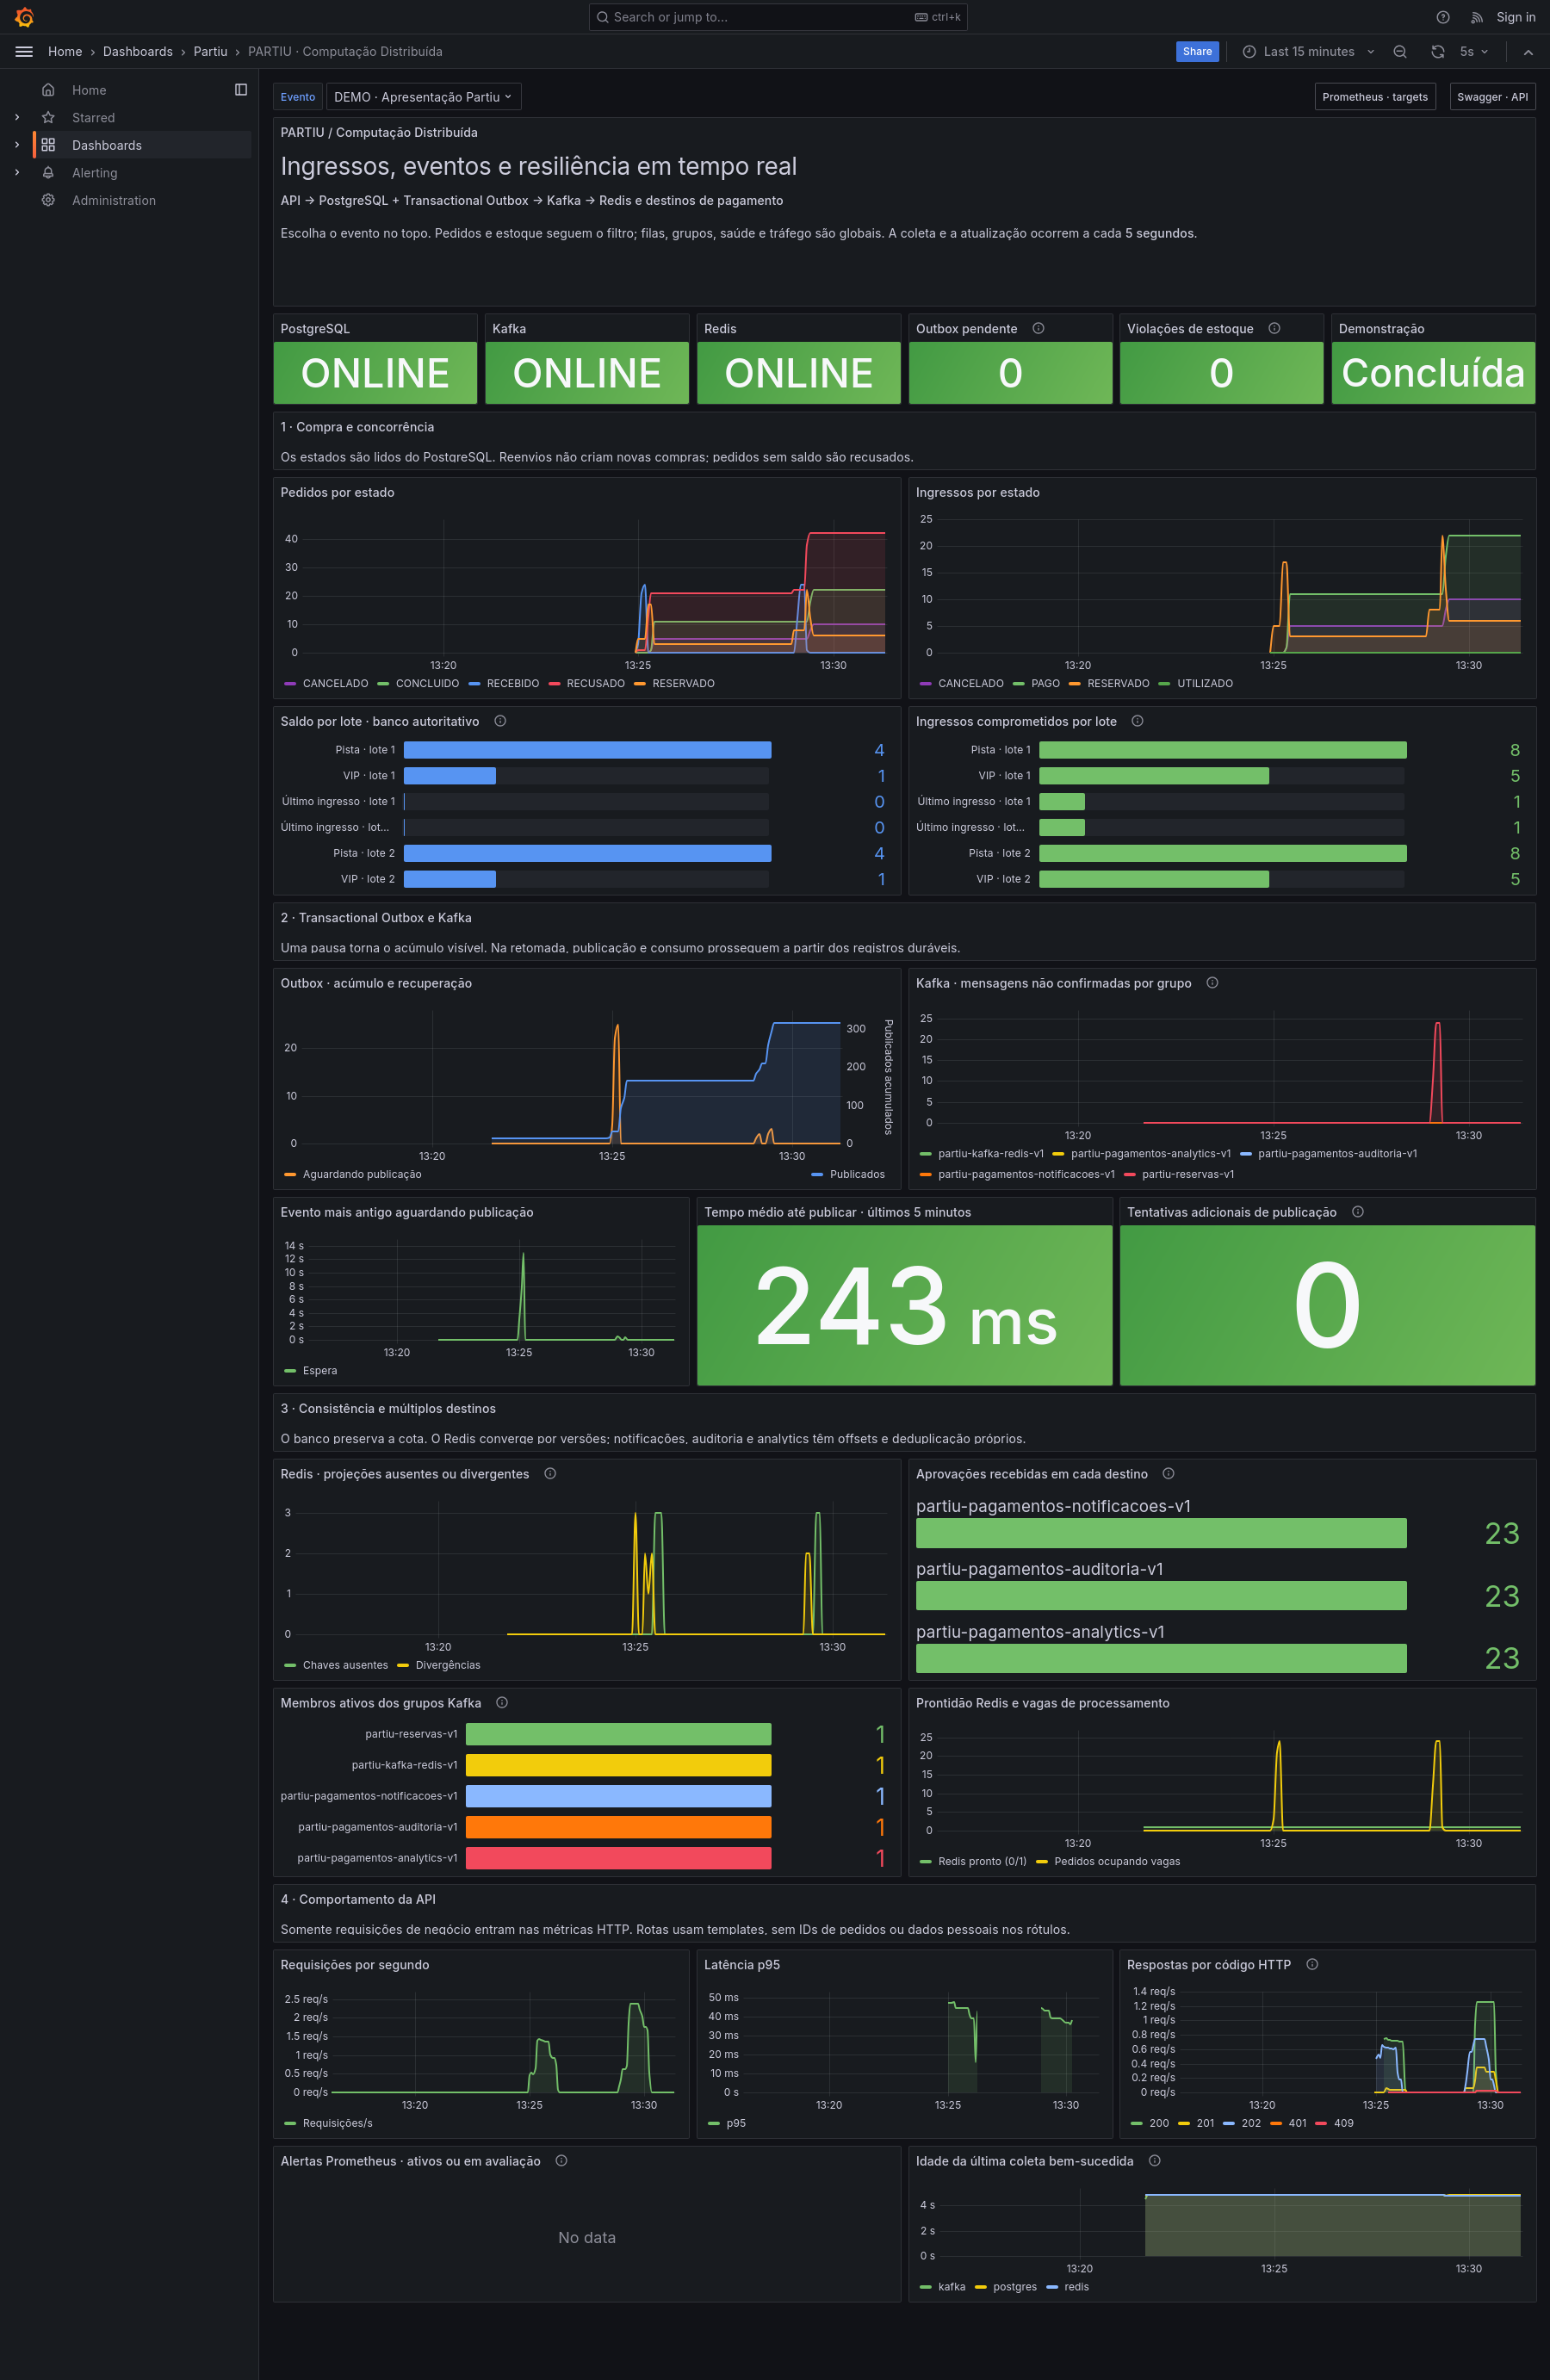
\includegraphics[width=\textwidth,height=0.92\textheight,keepaspectratio]{img/partiu-dashboard.png}
  \caption{Dashboard Grafana com m\'etricas reais da API e dos componentes distribu\'idos.}
\end{figure}

O dashboard organiza as evid\^encias em quatro grupos:

\begin{itemize}
  \item \textbf{Compra e concorr\^encia:} pedidos e ingressos por estado, saldo autoritativo por lote, ingressos comprometidos e viola\c{c}\~oes da cota. A m\'etrica de viola\c{c}\~ao deve permanecer em zero, pois a cota precisa ser igual ao saldo mais os ingressos ativos.
  \item \textbf{Transactional Outbox e Kafka:} quantidade de eventos aguardando publica\c{c}\~ao, idade do evento mais antigo, tempo de publica\c{c}\~ao, tentativas adicionais e lag por grupo consumidor.
  \item \textbf{Consist\^encia e m\'ultiplos destinos:} chaves Redis ausentes ou divergentes, vagas de processamento, membros ativos dos grupos e aprova\c{c}\~oes deduplicadas em notifica\c{c}\~oes, auditoria e analytics.
  \item \textbf{Comportamento da API:} requisi\c{c}\~oes por segundo, lat\^encia p95, c\'odigos HTTP e idade da \'ultima coleta. Falhas de coleta removem a medida da origem, em vez de apresent\'a-la indevidamente como zero.
\end{itemize}

O painel tamb\'em exibe a sa\'ude do PostgreSQL, Kafka e Redis, al\'em da etapa atual da demonstra\c{c}\~ao. As m\'etricas de sa\'ude e infraestrutura s\~ao globais; pedidos e estoque podem ser filtrados por evento. Essa distin\c{c}\~ao evita interpretar uma m\'etrica global como se fosse exclusiva de uma rodada de compra.

\subsection{Cen\'arios de demonstra\c{c}\~ao}

O ambiente local pode reproduzir falhas controladas para validar a resili\^encia:

\begin{enumerate}
  \item \textbf{Compra normal:} m\'ultiplas inten\c{c}\~oes disputam uma quantidade limitada de ingressos. O banco deve preservar a cota e recusar pedidos sem saldo.
  \item \textbf{Publicador pausado:} o \texttt{outbox-relay} \'e pausado por alguns segundos. A API continua persistindo pedidos e a outbox cresce, enquanto o Kafka ainda n\~ao recebe os eventos.
  \item \textbf{Recupera\c{c}\~ao:} com o publicador retomado, os eventos s\~ao drenados e os workers processam somente as unidades dispon\'iveis. A viola\c{c}\~ao de estoque deve continuar em zero.
  \item \textbf{Consumidor pausado:} ao pausar o \texttt{reservation-worker}, as mensagens chegam ao Kafka, o lag cresce e, ap\'os a retomada, o grupo recupera os pedidos e reduz o lag.
  \item \textbf{Reconstru\c{c}\~ao do Redis:} as proje\c{c}\~oes podem ser removidas para verificar se o consumidor ou a reconcilia\c{c}\~ao as reconstr\'oi a partir dos dados dur\'aveis do PostgreSQL.
\end{enumerate}

As regras do Prometheus alertam para depend\^encias indispon\'iveis, outbox antiga, viola\c{c}\~ao de cota, lag Kafka e diverg\^encia do Redis. Os alertas ficam vis\'iveis no ambiente de monitoramento, sem envio de notifica\c{c}\~oes externas durante a demonstra\c{c}\~ao.

\section{Autentica\c{c}\~ao e seguran\c{c}a}

A autentica\c{c}\~ao utiliza OAuth 2.0 com JWT:

\begin{enumerate}
  \item O usu\'ario entra com e-mail e senha ou por um provedor externo, como Google ou Facebook.
  \item O servi\c{c}o de autentica\c{c}\~ao emite um JWT com identidade e permiss\~oes.
  \item A API valida a assinatura e a validade do token localmente, sem consultar o banco em todas as requisi\c{c}\~oes.
  \item As permiss\~oes s\~ao verificadas antes de opera\c{c}\~oes como criar evento, editar lote ou consultar uma reserva.
\end{enumerate}

O gateway recebe apenas os dados necess\'arios para criar a cobran\c{c}a. Dados completos de cart\~ao devem permanecer no ambiente do provedor, reduzindo a responsabilidade do PARTIU sobre informa\c{c}\~oes financeiras sens\'iveis.

\section{Prot\'otipo desenvolvido}

Nesta etapa do projeto, foi desenvolvido um prot\'otipo naveg\'avel do fluxo principal de compra. A interface foi pensada para conduzir o comprador desde a descoberta de um evento at\'e a escolha do ingresso e o pagamento, mantendo claras as informa\c{c}\~oes de disponibilidade, pre\c{c}o e estado da compra. As telas tamb\'em servir\~ao como base para os testes de carga e de concorr\^encia da plataforma distribu\'ida.

\subsection{Entrada e descoberta de eventos}

\begin{figure}[H]
  \centering
  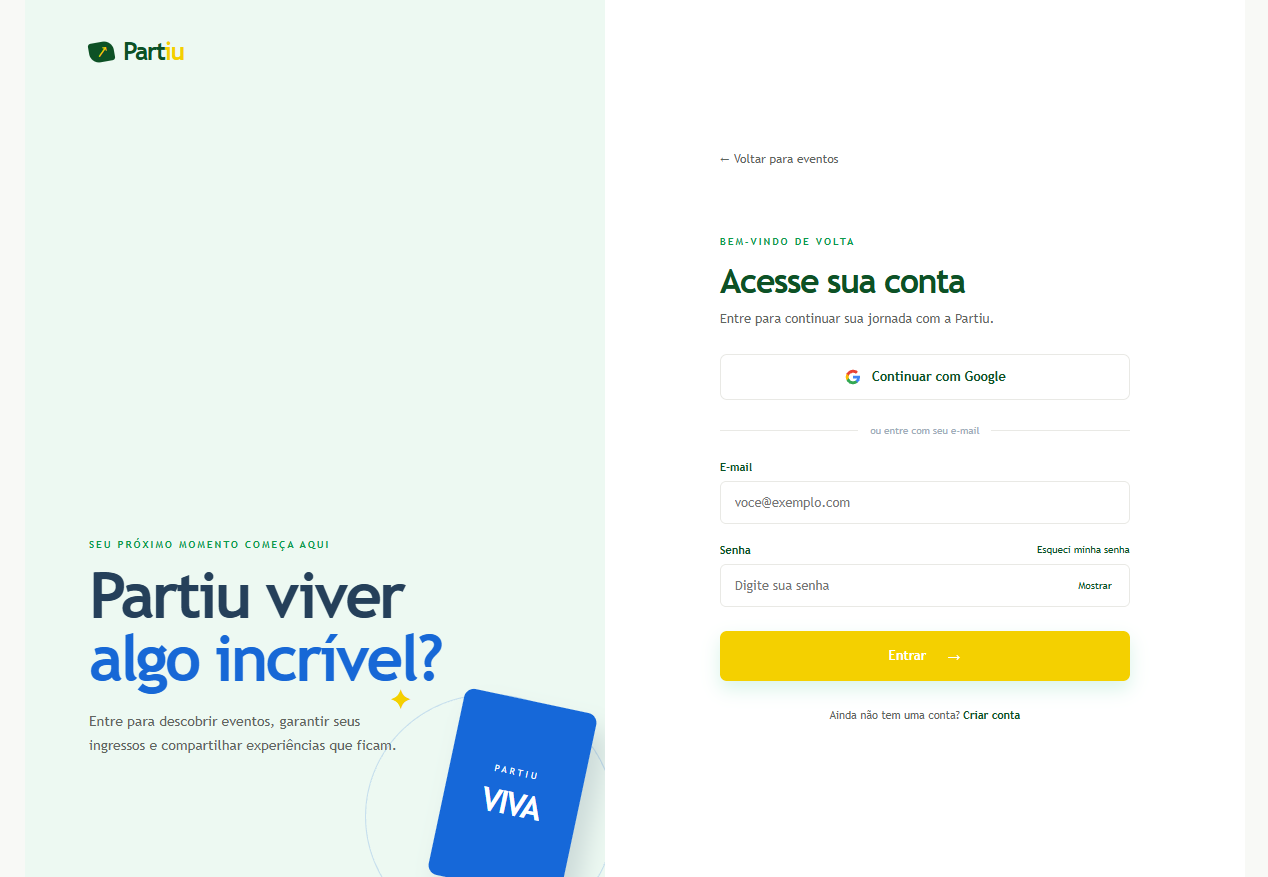
\includegraphics[width=\textwidth,height=0.72\textheight,keepaspectratio]{img/auth.png}
  \caption{Tela de autentica\c{c}\~ao do comprador.}
\end{figure}

A autentica\c{c}\~ao antecede as opera\c{c}\~oes que alteram estoque. Depois de entrar, o usu\'ario acessa a p\'agina inicial, que apresenta a busca e os eventos publicados.

\begin{figure}[H]
  \centering
  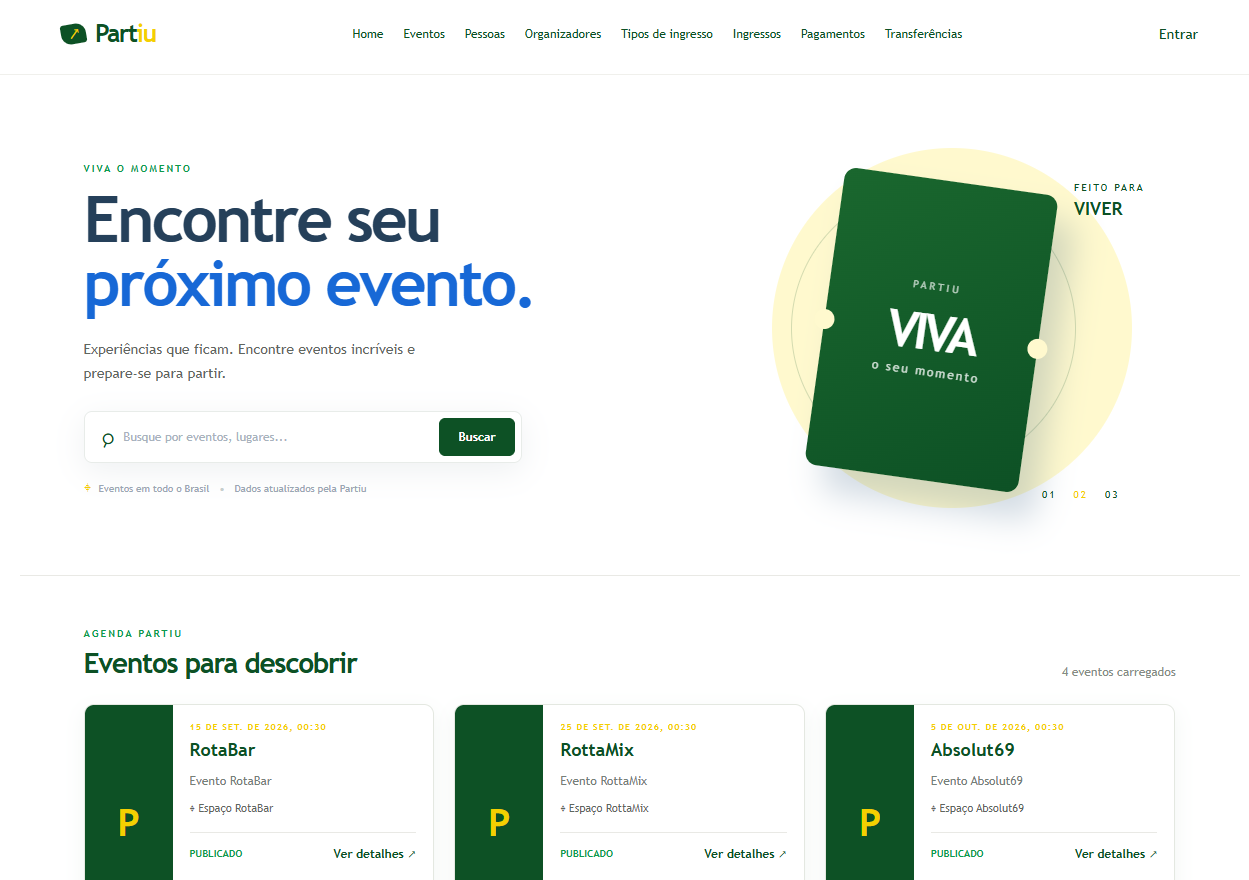
\includegraphics[width=\textwidth,height=0.78\textheight,keepaspectratio]{img/home.png}
  \caption{P\'agina inicial com busca e lista de eventos.}
\end{figure}

\subsection{Detalhes do evento e sele\c{c}\~ao do ingresso}

\begin{figure}[H]
  \centering
  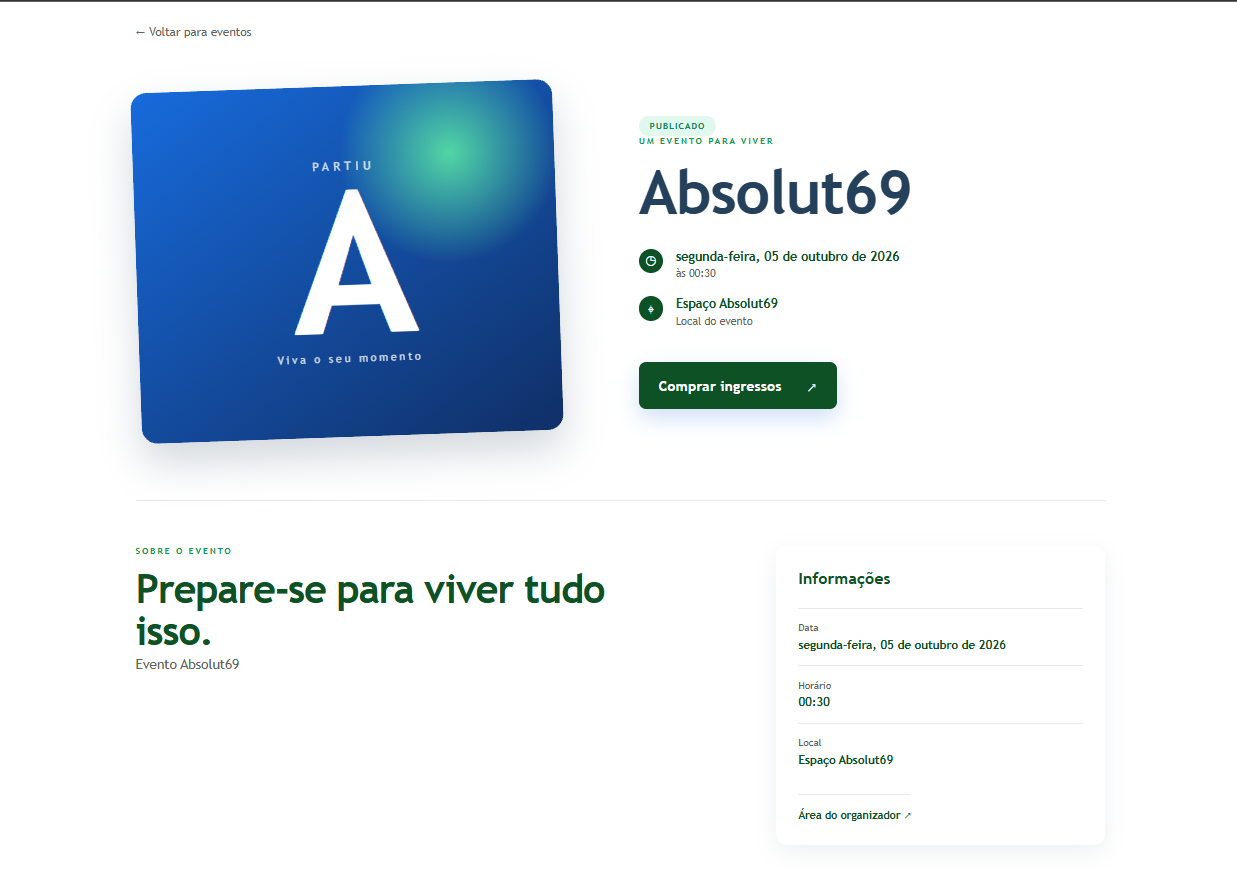
\includegraphics[width=\textwidth,height=0.78\textheight,keepaspectratio]{img/evento.png}
  \caption{P\'agina de detalhes do evento.}
\end{figure}

Na p\'agina de detalhes, o comprador visualiza data, hor\'ario, local e o bot\~ao de compra. Ao avan\c{c}ar, a interface apresenta os tipos de ingresso, seus lotes, pre\c{c}os e quantidade dispon\'ivel.

\begin{figure}[H]
  \centering
  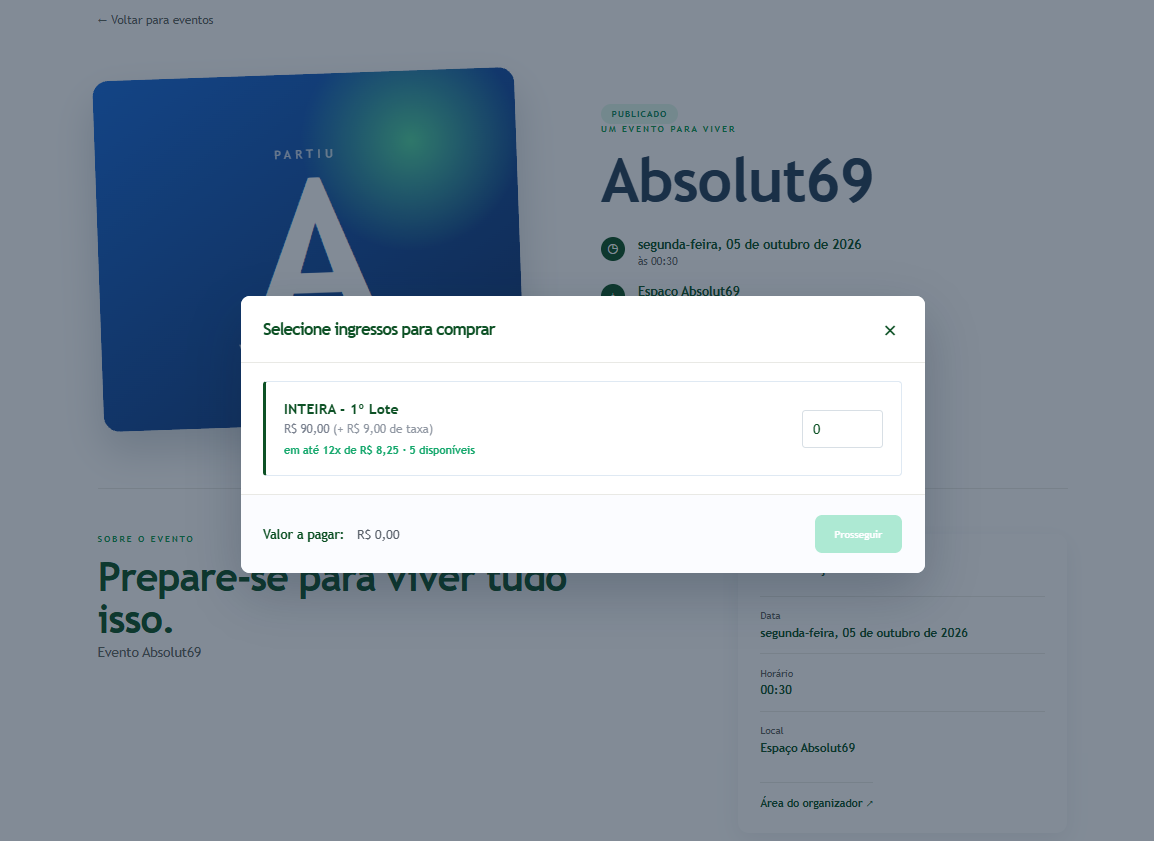
\includegraphics[width=\textwidth,height=0.78\textheight,keepaspectratio]{img/tipoIngresso.png}
  \caption{Modal de sele\c{c}\~ao do tipo e da quantidade de ingressos.}
\end{figure}

Essa etapa \'e o primeiro ponto cr\'itico para a concorr\^encia: a quantidade exibida \'e informativa e pode mudar enquanto a tela est\'a aberta. A confirma\c{c}\~ao real ocorre no servidor, que revalida o lote e registra a reserva de forma at\^omica.

\subsection{Pagamento}

\begin{figure}[H]
  \centering
  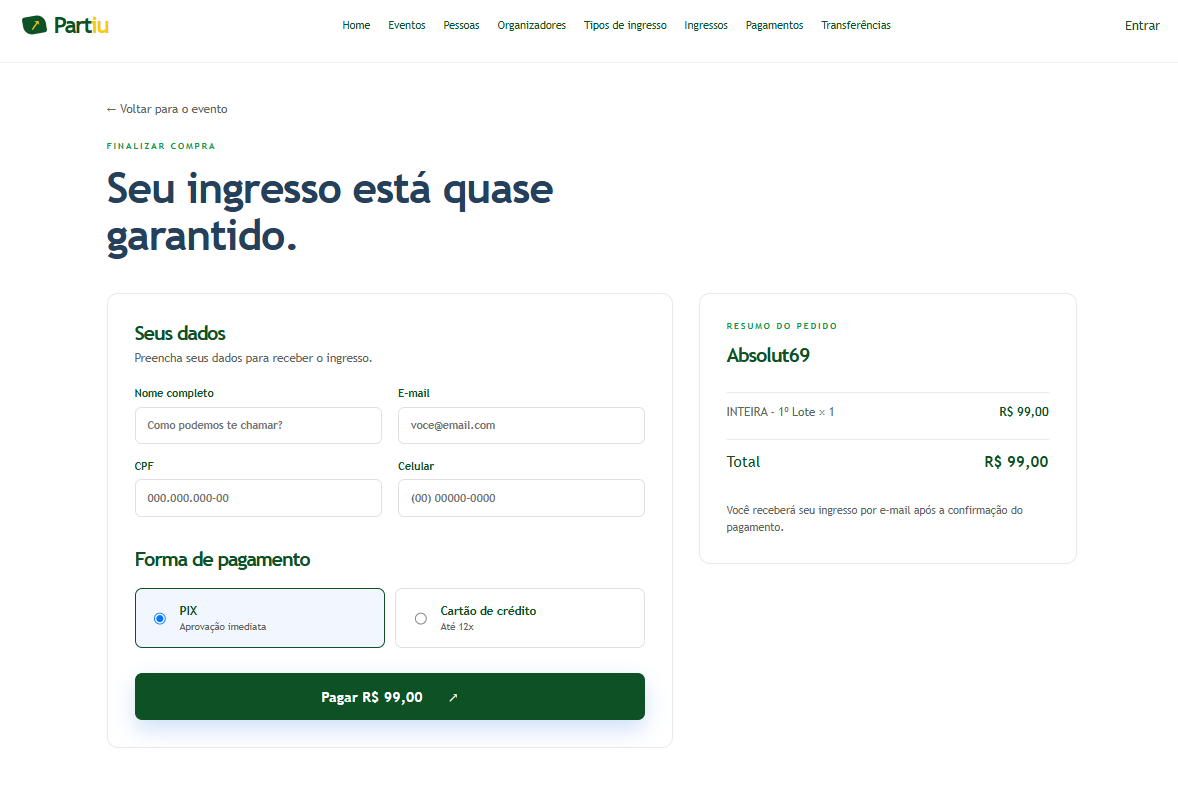
\includegraphics[width=\textwidth,height=0.78\textheight,keepaspectratio]{img/pagamento.png}
  \caption{Tela de preenchimento dos dados e escolha do meio de pagamento.}
\end{figure}

Na tela de pagamento, os dados pessoais s\~ao associados \`a compra e o comprador escolhe PIX ou cart\~ao. O bot\~ao de pagamento n\~ao deve considerar o ingresso definitivamente vendido apenas por ter sido acionado: a aplica\c{c}\~ao cria uma inten\c{c}\~ao idempotente, preserva a reserva tempor\'aria e aguarda a confirma\c{c}\~ao do gateway.

\subsection{Como o prot\'otipo ser\'a testado}

\begin{itemize}
  \item \textbf{Fluxo funcional:} autenticar, localizar um evento, escolher um lote, informar os dados e iniciar o pagamento.
  \item \textbf{Concorr\^encia:} enviar requisi\c{c}\~oes simult\^aneas para o mesmo lote e verificar que a soma de ingressos \texttt{RESERVADO} e \texttt{PAGO} nunca ultrapassa a cota.
  \item \textbf{Repeti\c{c}\~ao:} reenviar a mesma requisi\c{c}\~ao ou webhook e verificar que a chave idempotente impede reservas e cobran\c{c}as duplicadas.
  \item \textbf{Falhas:} interromper consumidores, atrasar o gateway e indisponibilizar o Redis para observar respostas \texttt{429}/\texttt{503}, reprocessamento da fila e recupera\c{c}\~ao sem venda duplicada.
  \item \textbf{Expira\c{c}\~ao:} abandonar o checkout e confirmar que uma rotina libera reservas vencidas, devolve o estoque uma \'unica vez e n\~ao deixa ingressos bloqueados permanentemente.
\end{itemize}

\section{Entidades do dom\'inio}

\begin{longtable}{>{\bfseries}p{3.2cm}p{10.1cm}}
\toprule
Entidade & Responsabilidade \\
\midrule
Pessoa & Cadastro de compradores e organizadores, com nome, e-mail, CPF e credenciais protegidas. \\
Organizador & Associa\c{c}\~ao entre uma pessoa e um evento, incluindo permiss\~oes de gest\~ao. \\
Evento & Nome, descri\c{c}\~ao, data, local e status do evento. \\
TipoIngresso & Categoria ou lote, como Pista, VIP, Camarote ou Bistr\^o, com pre\c{c}o, cota total e saldo dispon\'ivel. \\
Ingresso & Unidade associada \`a pessoa e ao tipo de ingresso, com status da reserva, pagamento e QR Code. \\
Pagamento & Identificador da cobran\c{c}a no gateway, valor, status, timestamps e chave de idempot\^encia. \\
Transferencia & Registro de transfer\^encia de titularidade de um ingresso, quando essa opera\c{c}\~ao for permitida. \\
\bottomrule
\end{longtable}

\section{Fluxo detalhado de compra}

\subsection{Estados da reserva}

\texttt{reservado} $\rightarrow$ \texttt{aguardando\_pagamento} $\rightarrow$ \texttt{pago}

Uma reserva tamb\'em pode seguir para \texttt{cancelado} por falha no pagamento, cancelamento expl\'icito ou expira\c{c}\~ao do prazo. A devolu\c{c}\~ao do estoque deve ser executada uma \^unica vez, dentro de uma opera\c{c}\~ao transacional ou protegida por idempot\^encia.

\begin{enumerate}
  \item O comprador escolhe o evento e o lote. A API valida o JWT, o pre\c{c}o vigente e a disponibilidade.
  \item A inten\c{c}\~ao de compra recebe um identificador idempotente e \'e publicada na fila. O cliente recebe um status de processamento.
  \item A API solicita ao Redis uma permiss\~ao limitada por lote. Se a capacidade segura estiver esgotada ou o Redis estiver indispon\'ivel, responde rapidamente com \texttt{429} ou \texttt{503}, sem publicar na fila nem acessar o banco.
  \item Somente pedidos admitidos entram na fila. O worker executa no banco uma atualiza\c{c}\~ao condicional, como:
\end{enumerate}

\begin{lstlisting}[language=SQL]
UPDATE tipos_ingresso
SET qtd_disponivel = qtd_disponivel - 1
WHERE id = :tipo_ingresso_id AND qtd_disponivel > 0;
\end{lstlisting}

Se a baixa for aceita, o sistema cria uma reserva com prazo de expira\c{c}\~ao. Se n\~ao houver saldo, a solicita\c{c}\~ao \'e recusada sem alterar o estoque.

O servi\c{c}o de pagamentos cria uma cobran\c{c}a no gateway e associa o identificador externo \`a reserva. O gateway processa o pagamento e envia um webhook assinado quando a cobran\c{c}a muda de estado. A API valida assinatura, valor e identificadores e processa o evento de forma idempotente.

Em caso de pagamento aprovado, a reserva vira \texttt{pago} e o QR Code \'e liberado. Em caso de falha, cancelamento ou expira\c{c}\~ao, a reserva vira \texttt{cancelado} e o saldo retorna ao lote.

\section{Concorr\^encia e alta disponibilidade}

O controle contra \textit{double selling} combina tr\^es mecanismos, com responsabilidades diferentes:

\begin{itemize}
  \item \textbf{Fila de mensageria:} Kafka absorve picos e distribui pedidos entre trabalhadores.
  \item \textbf{Admission control fail fast:} Redis limita a quantidade de pedidos do mesmo lote que podem avan\c{c}ar para a fila e o worker.
  \item \textbf{Atualiza\c{c}\~ao at\^omica:} o banco s\'o reduz a quantidade quando o saldo ainda \'e maior que zero, preservando a consist\^encia ACID.
\end{itemize}

O Redis n\~ao \'e fonte de estoque e n\~ao substitui a restri\c{c}\~ao do banco. Ele controla press\~ao e aplica \textit{fail fast}; a atualiza\c{c}\~ao condicional \'e a garantia final de consist\^encia. A permiss\~ao deve ter TTL e ser liberada pelo worker em \texttt{finally}, inclusive quando a transa\c{c}\~ao falha. A API e os trabalhadores podem ser replicados atr\'as de um balanceador; Redis, banco e fila devem ser executados com redund\^ancia e monitoramento.

\subsection{Escritas seguras e expira\c{c}\~ao}

Cada tentativa de compra ter\'a uma chave idempotente persistida. A transa\c{c}\~ao de reserva deve validar o estado atual, reduzir o estoque somente com saldo positivo e criar o ingresso com \texttt{expires\_at}. Uma restri\c{c}\~ao de unicidade para a chave da inten\c{c}\~ao impede que o mesmo pedido seja aplicado duas vezes, mesmo que a mensagem Kafka seja entregue novamente.

Um processo de expira\c{c}\~ao busca reservas vencidas usando bloqueio compat\'ivel com o banco, altera somente registros ainda em \texttt{RESERVADO} ou \texttt{AGUARDANDO\_PAGAMENTO} e, na mesma transa\c{c}\~ao, devolve a unidade ao lote. Assim, uma reserva j\'a paga n\~ao \'e cancelada por engano e uma reserva abandonada n\~ao permanece ocupando estoque. A transi\c{c}\~ao de estado e a devolu\c{c}\~ao devem ser idempotentes, para que uma nova tentativa ap\'os uma falha n\~ao duplique o saldo.

\section{Casos de uso principais}

\begin{itemize}
  \item \textbf{Criar e gerenciar evento:} o organizador cadastra o evento e configura categorias, lotes, pre\c{c}os e cotas.
  \item \textbf{Reservar ingresso:} o comprador seleciona uma categoria e obt\'em uma reserva tempor\'aria se houver saldo.
  \item \textbf{Pagar:} o sistema cria a cobran\c{c}a no gateway e acompanha o resultado sem expor dados de cart\~ao ao PARTIU.
  \item \textbf{Confirmar pagamento:} o webhook validado altera a reserva para paga e libera o QR Code.
  \item \textbf{Expirar reserva:} um processo peri\'odico identifica reservas vencidas, cancela a cobran\c{c}a quando aplic\'avel e devolve a unidade ao lote.
  \item \textbf{Validar acesso:} a equipe do evento consulta ou l\^e o QR Code e verifica se o ingresso est\'a pago e ainda n\~ao foi utilizado.
\end{itemize}

\section{Diagramas do projeto}

\subsection{Casos de uso}
\begin{figure}[H]
  \centering
  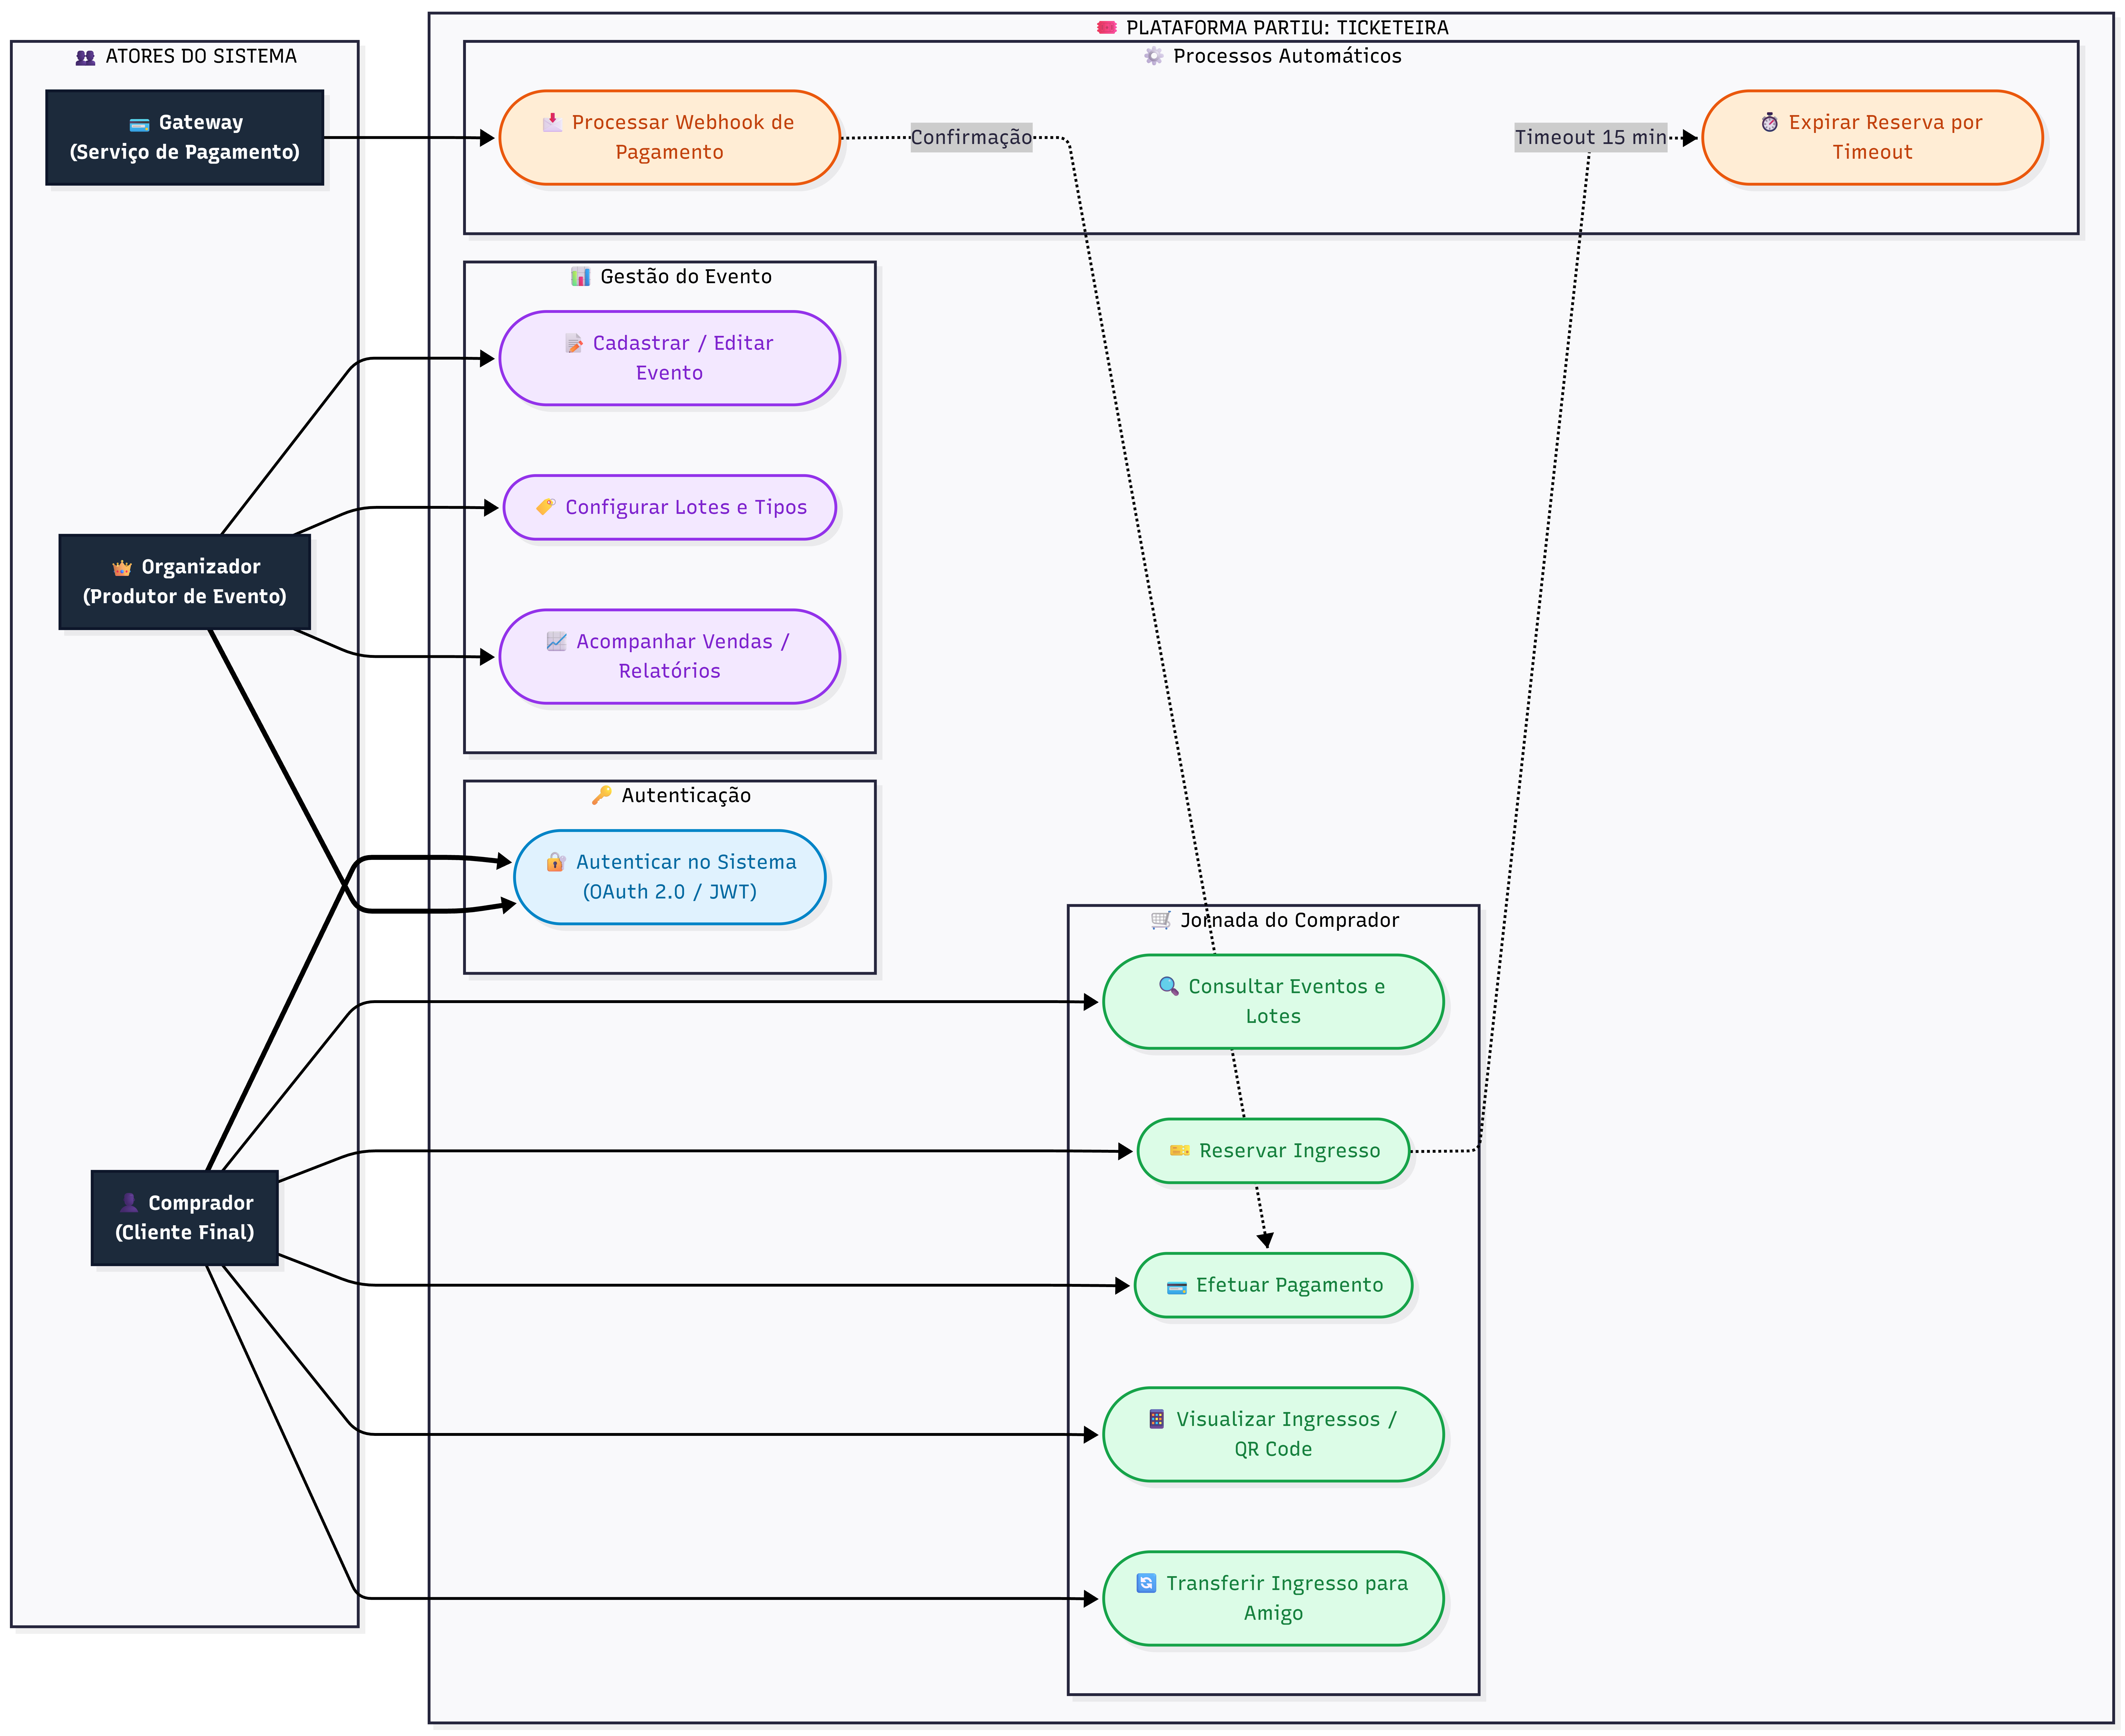
\includegraphics[width=\textwidth,height=0.78\textheight,keepaspectratio]{Casos de uso-2026-09-01-161103.png}
  \caption{Casos de uso do sistema.}
\end{figure}

Este diagrama apresenta os atores e as funcionalidades externas do sistema: compradores, organizadores, operadores e gateway de pagamento.

\subsection{Modelo de arquitetura}
\begin{figure}[H]
  \centering
  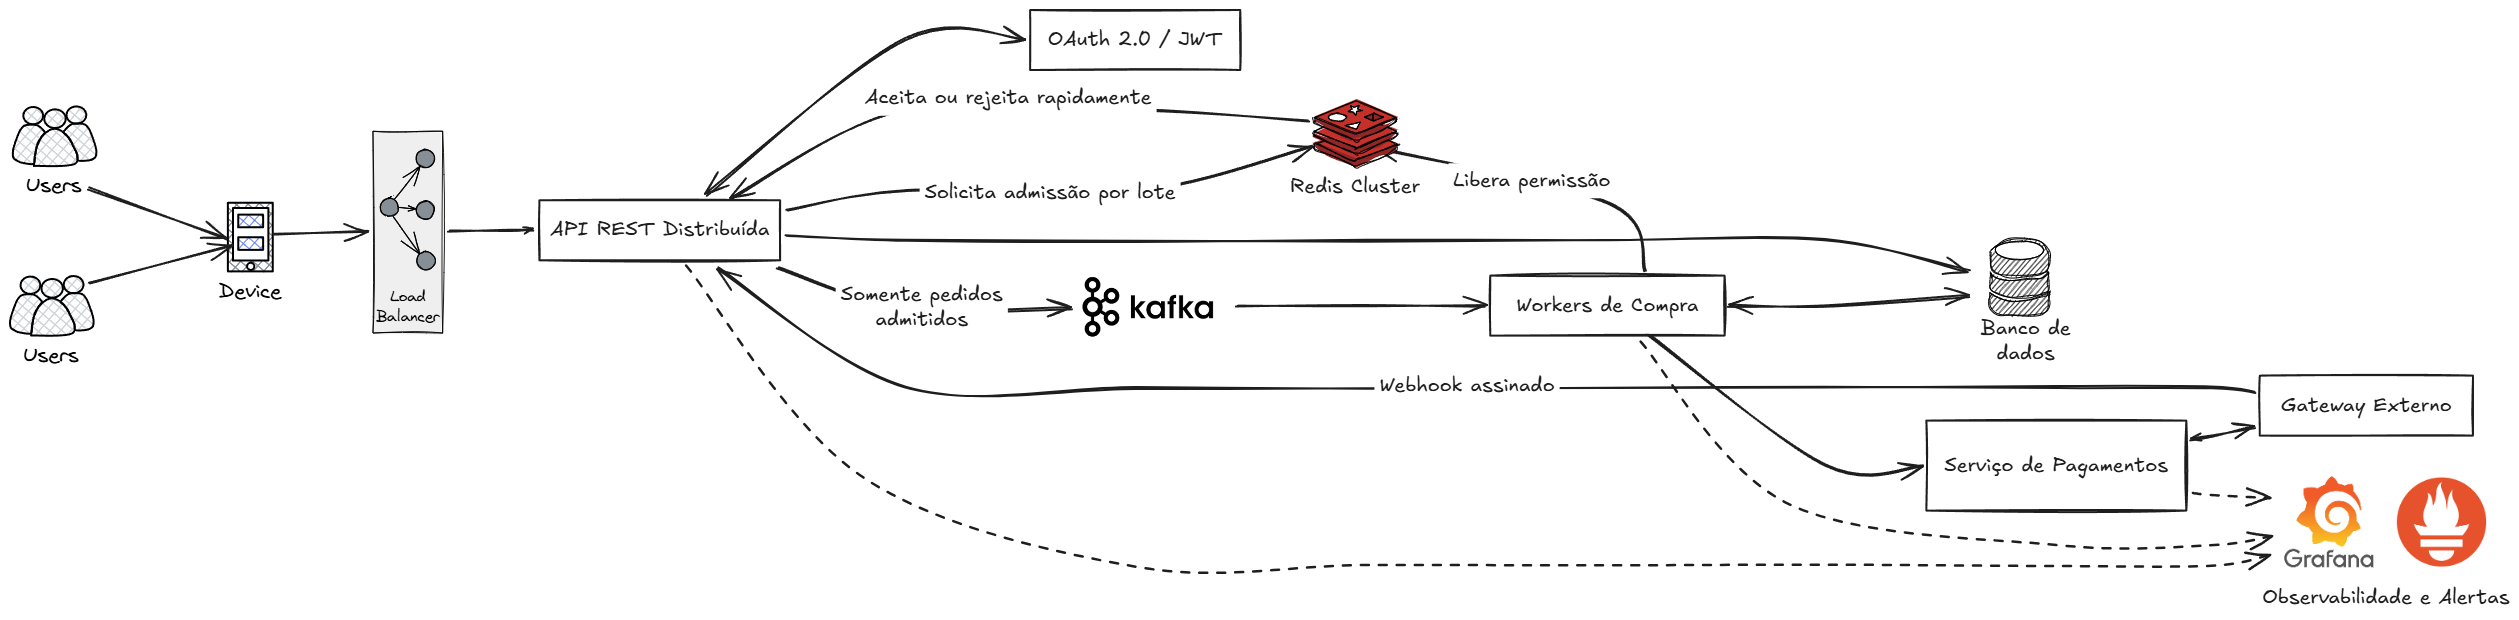
\includegraphics[width=\textwidth,height=0.82\textheight,keepaspectratio]{Modelo 1.png}
  \caption{Modelo de arquitetura do PARTIU.}
\end{figure}

O modelo mostra a divis\~ao em interface, servi\c{c}os de aplica\c{c}\~ao e persist\^encia. A fronteira entre a aplica\c{c}\~ao e as integra\c{c}\~oes externas evidencia que autentica\c{c}\~ao e pagamentos podem evoluir sem acoplar a interface ao banco.

\subsection{Fluxo distribu\'ido de compra}
\begin{figure}[H]
  \centering
  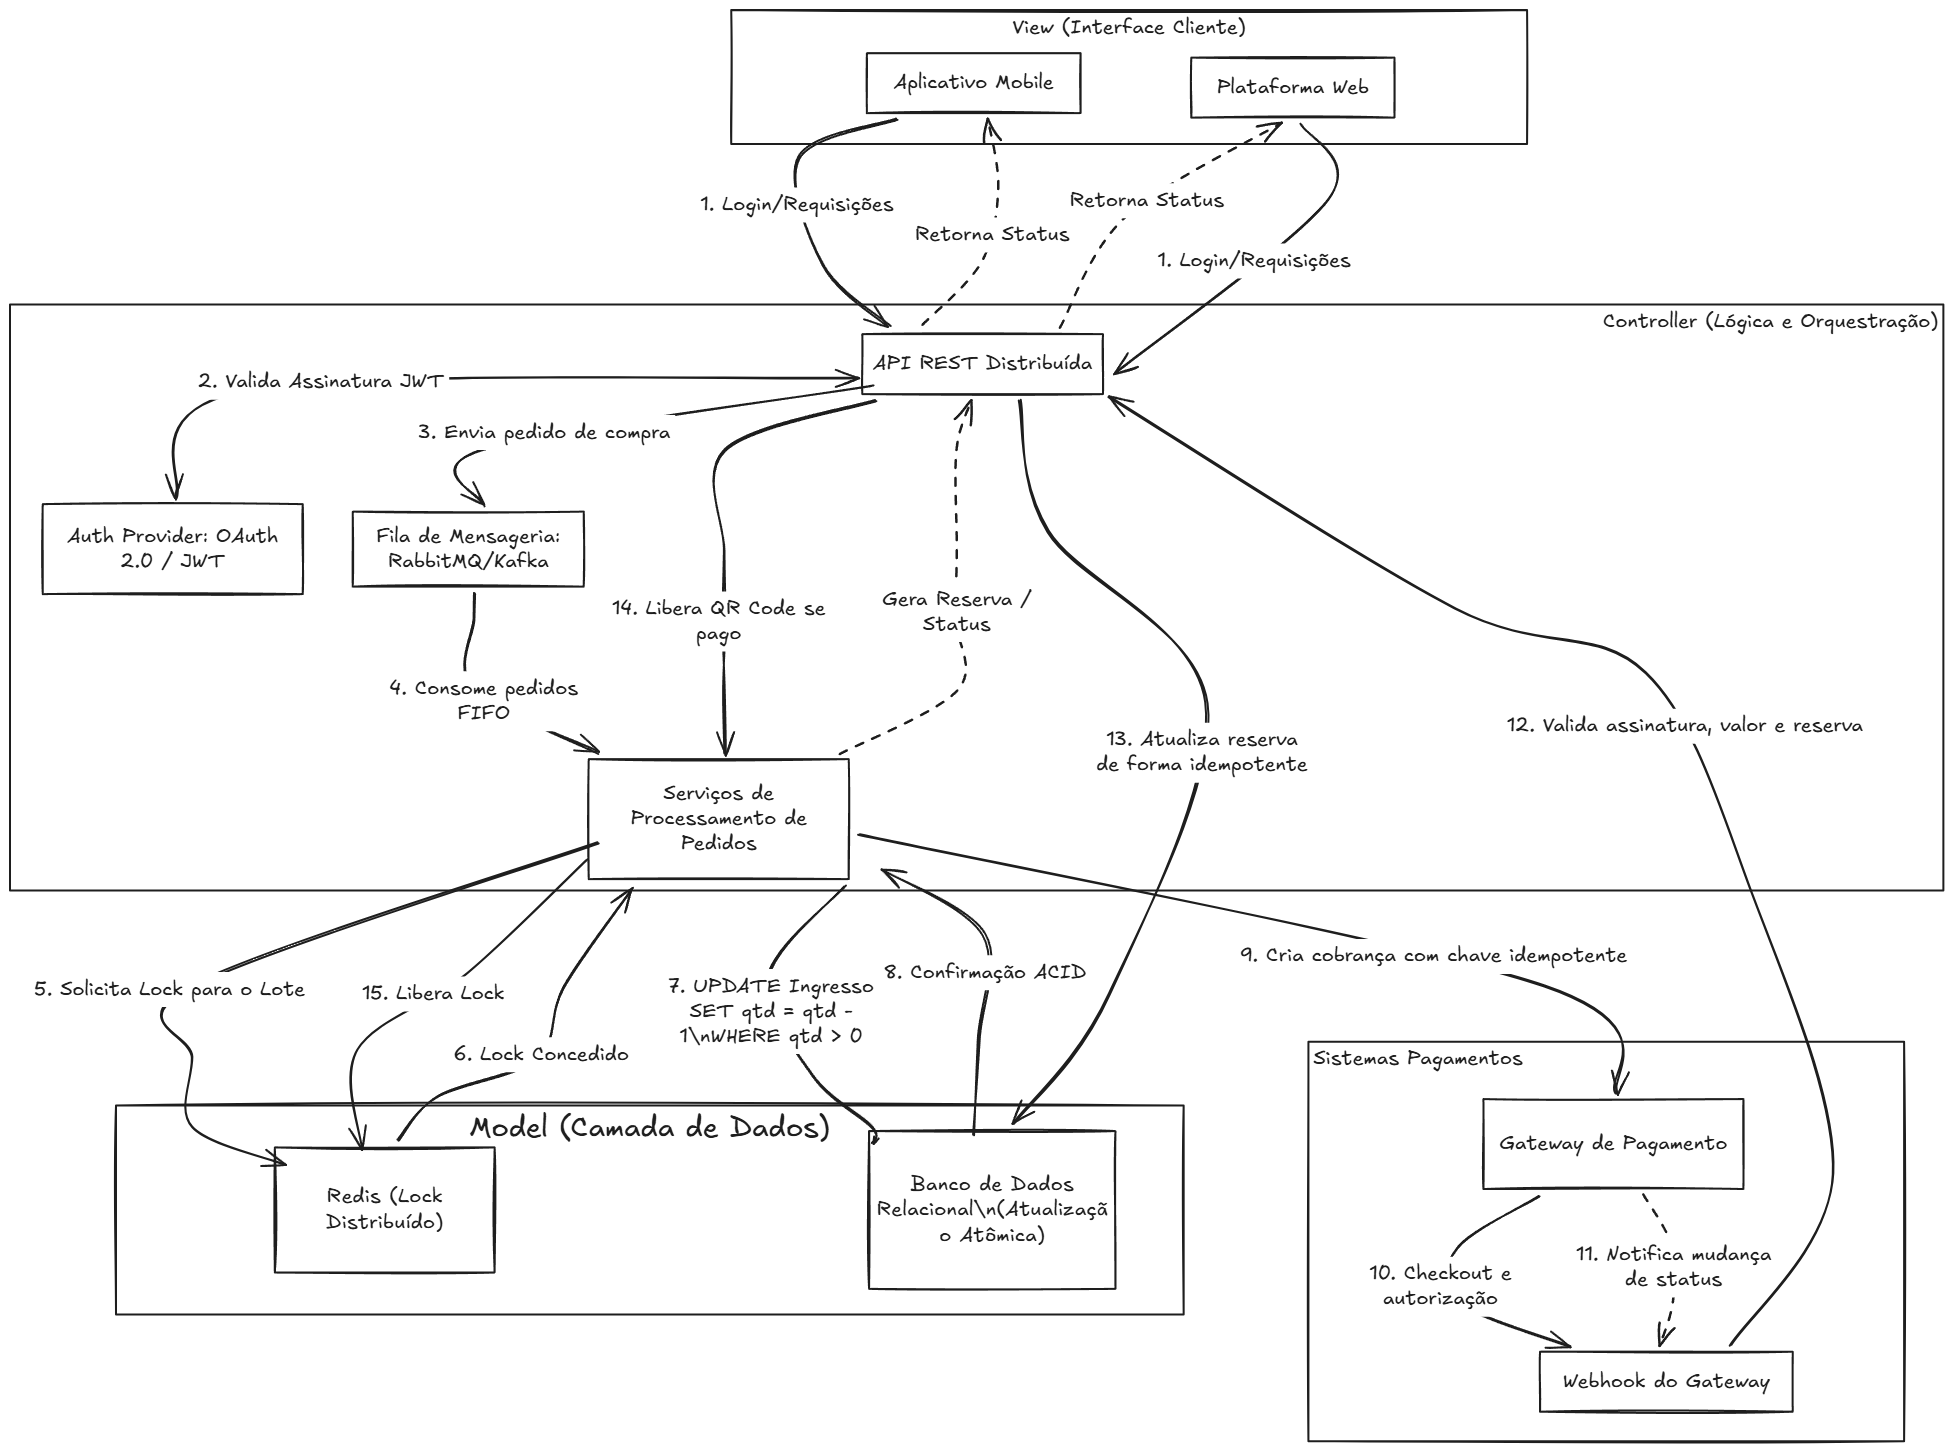
\includegraphics[width=\textwidth,height=0.82\textheight,keepaspectratio]{modelo 2.png}
  \caption{Fluxo distribu\'ido de compra.}
\end{figure}

Este desenho detalha o caminho cr\'itico entre cliente, API, autentica\c{c}\~ao, fila, trabalhador, Redis e banco relacional. O pagamento n\~ao baixa o estoque diretamente: a unidade \'e reservada antes, e s\'o a confirma\c{c}\~ao validada libera o ingresso.

\subsubsection*{Responsabilidade de cada etapa}
\begin{enumerate}
  \item \textbf{Cliente -> API:} o aplicativo ou a plataforma web envia evento, lote, quantidade e chave idempotente. A API valida o JWT, os par\^ametros, o pre\c{c}o vigente e a permiss\~ao do comprador.
  \item \textbf{API -> Auth Provider:} a API valida assinatura, expira\c{c}\~ao e escopos do JWT. Token inv\'alido deve ser rejeitado antes de publicar qualquer pedido.
  \item \textbf{API -> Redis:} a API solicita uma permiss\~ao de admiss\~ao para o \texttt{tipo\_ingresso\_id}. O Redis mant\'em um contador ou sem\'aforo limitado, com TTL.
  \item \textbf{Redis -> API:} se houver capacidade, confirma a permiss\~ao; se o limite estiver atingido ou estiver indispon\'ivel, a API responde com \texttt{429} ou \texttt{503}.
  \item \textbf{API -> Fila:} somente depois da admiss\~ao confirmada a API registra a inten\c{c}\~ao e publica mensagem dur\'avel. Se a publica\c{c}\~ao falhar, a permiss\~ao retorna ao Redis.
  \item \textbf{Fila -> Worker:} o worker consome pedidos admitidos e confirma a mensagem somente depois de concluir a reserva e criar ou reconhecer a cobran\c{c}a.
  \item \textbf{Worker -> Banco:} executa a atualiza\c{c}\~ao condicional em uma transa\c{c}\~ao. O Redis n\~ao informa nem substitui o saldo real.
  \item \textbf{Banco -> Worker:} uma linha atualizada confirma a baixa; nenhuma linha significa lote esgotado. O worker cria a reserva \texttt{RESERVADO} com prazo de expira\c{c}\~ao.
  \item \textbf{Worker -> Gateway:} cria a cobran\c{c}a usando \texttt{idempotency\_key}, valor calculado no servidor e refer\^encia da reserva.
  \item \textbf{Gateway -> Checkout:} processa PIX, d\'ebito, cr\'edito ou outro meio suportado. Criar a cobran\c{c}a significa apenas \texttt{PENDENTE}.
  \item \textbf{Gateway -> Webhook:} envia evento assinado com \texttt{event\_id}, status, valor e identificador externo. Reenvios s\~ao esperados.
  \item \textbf{Webhook -> API:} valida assinatura, gateway, \texttt{event\_id}, valor, \texttt{gateway\_payment\_id} e v\'inculo com o pagamento.
  \item \textbf{API -> Banco:} em uma transa\c{c}\~ao, altera pagamento e ingresso apenas se o estado permitir a transi\c{c}\~ao. Evento repetido n\~ao cria ingresso nem devolve estoque novamente.
  \item \textbf{API -> Worker:} pagamento aprovado libera o QR Code; falha, cancelamento ou expira\c{c}\~ao marca o ingresso como \texttt{CANCELADO} e devolve a unidade uma \^unica vez.
  \item \textbf{Worker -> Redis:} ap\'os persistir o resultado, inclusive em erro, libera a permiss\~ao em um bloco \texttt{finally}. O TTL protege contra queda do processo.
  \item \textbf{API -> Cliente:} retorna o estado por consulta, polling ou notifica\c{c}\~ao. O cliente s\'o exibe o QR Code quando o estado persistido for \texttt{PAGO}.
\end{enumerate}

\subsection{Modelo de dados}
\begin{figure}[H]
  \centering
  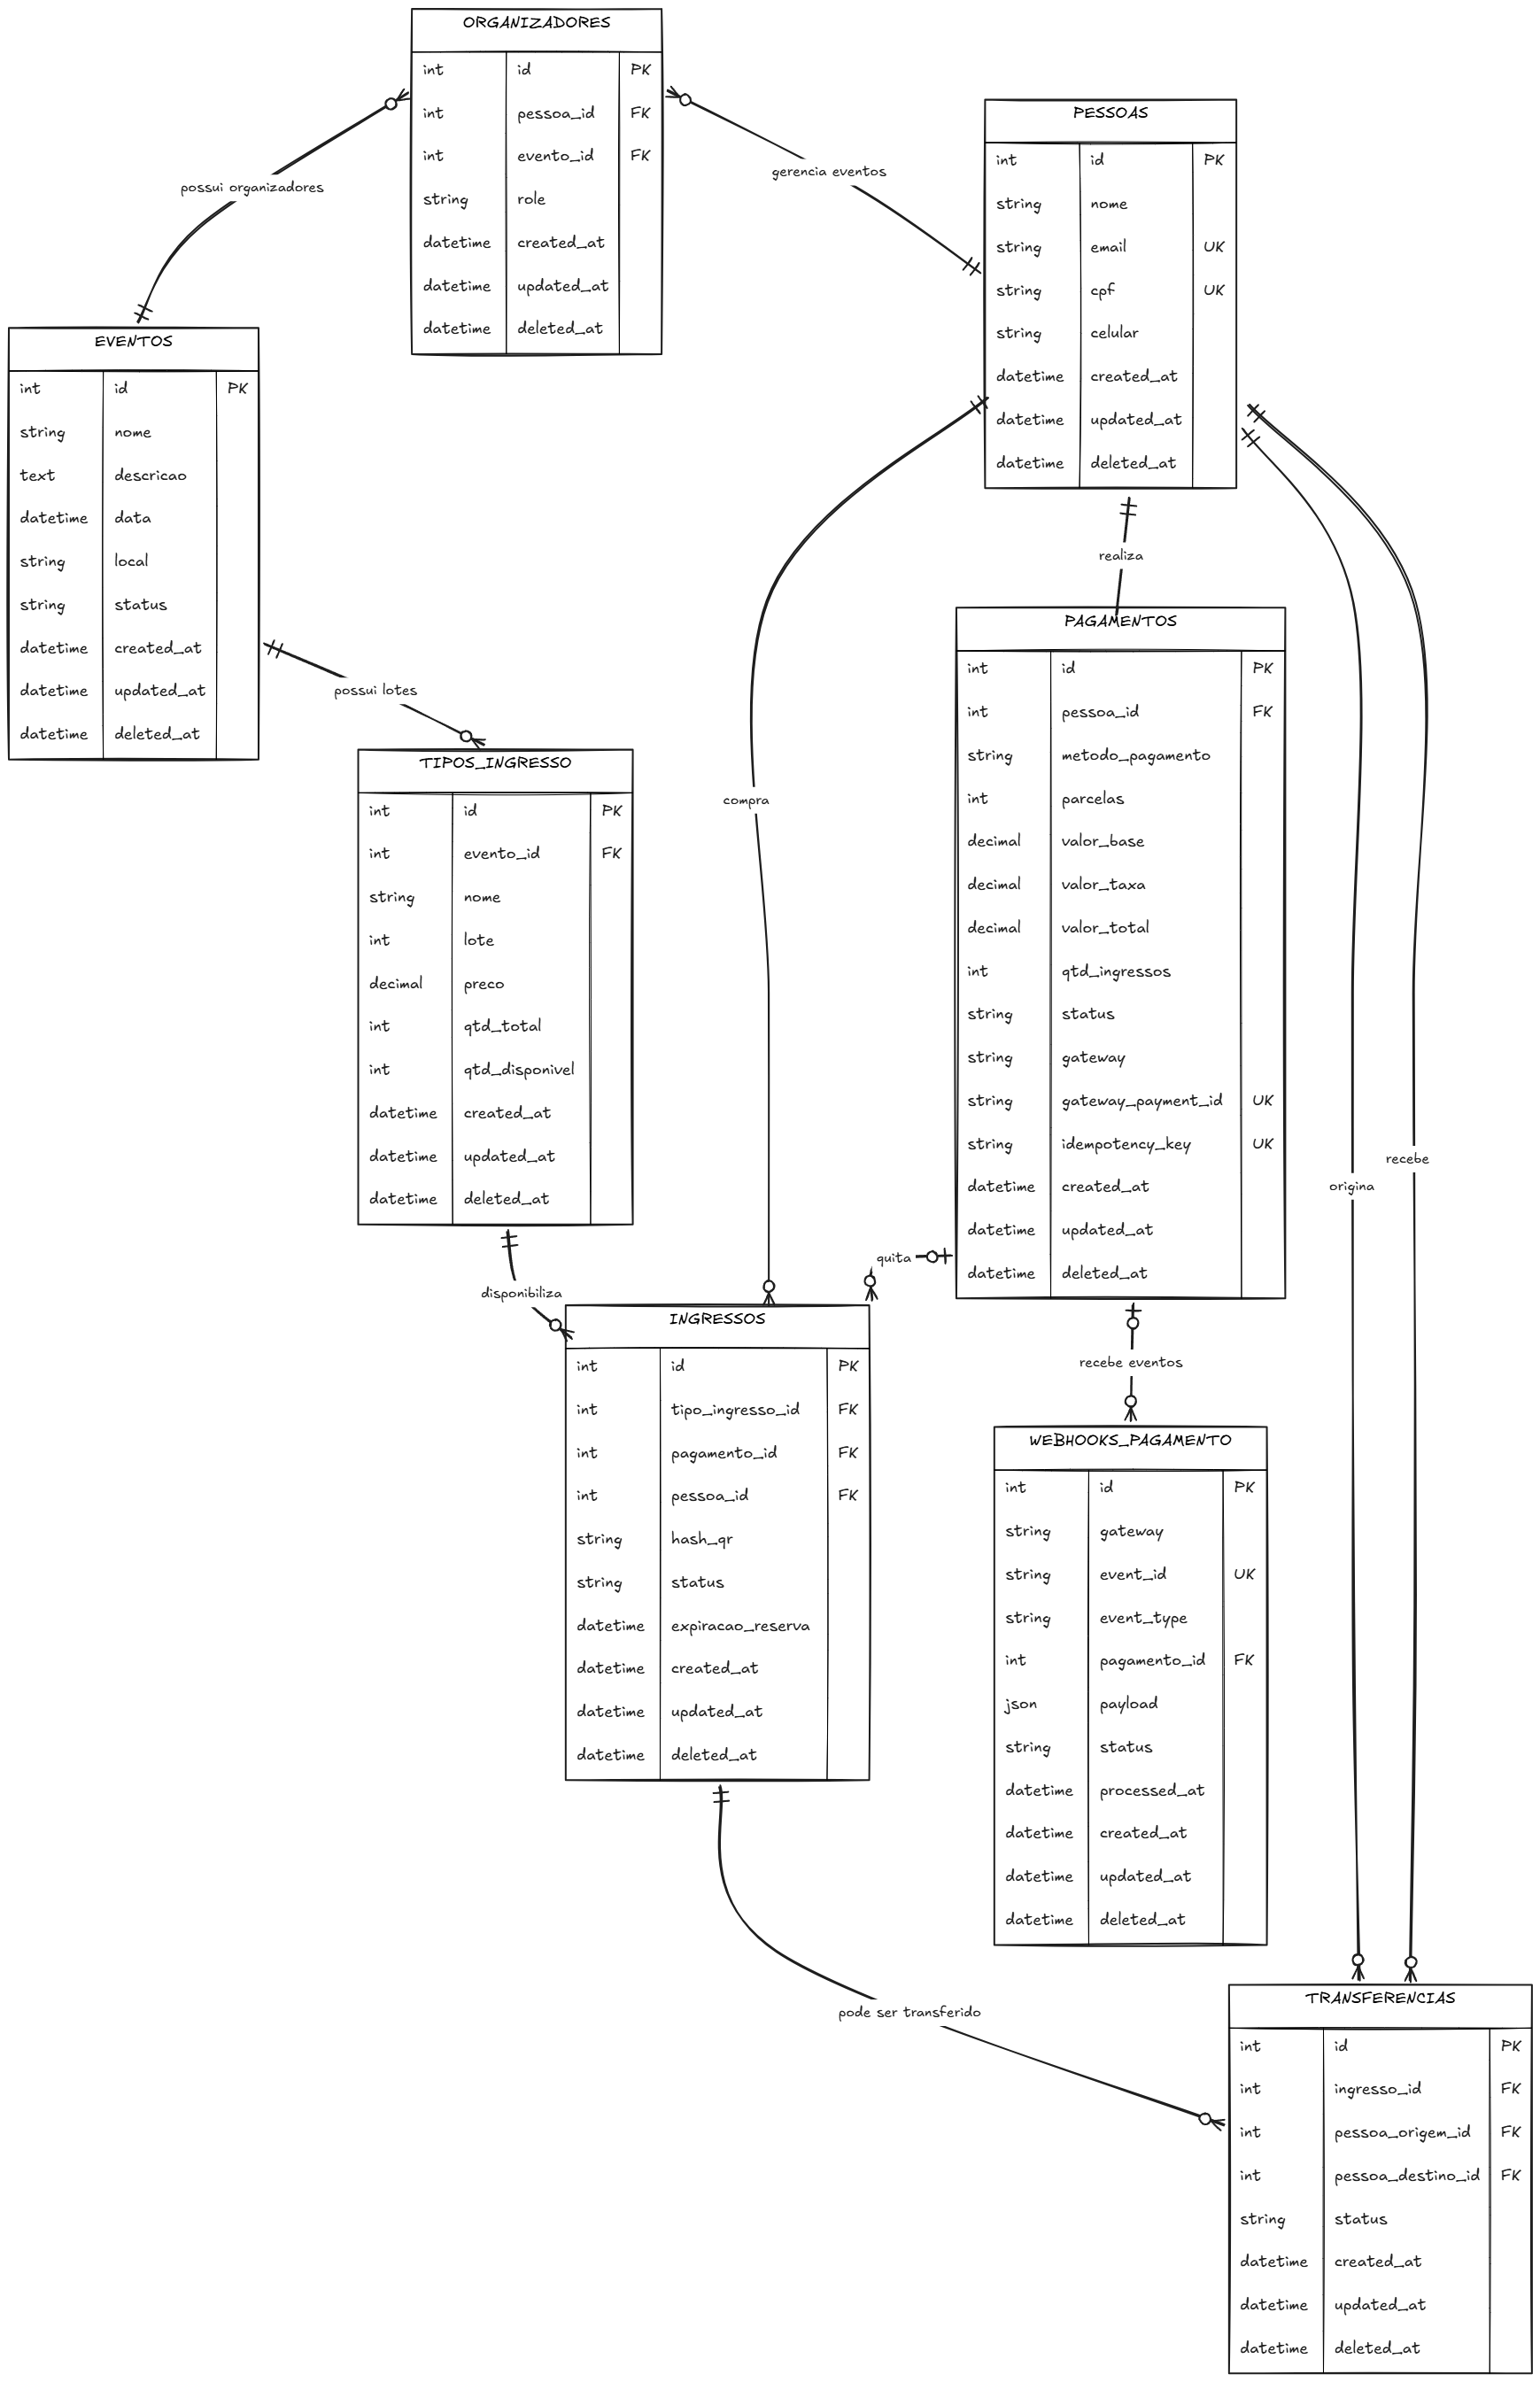
\includegraphics[width=\textwidth,height=0.93\textheight,keepaspectratio]{PARTIU_DIAGRAM_DB.png}
  \caption{Modelo de dados do PARTIU.}
\end{figure}

O diagrama de banco representa as entidades e seus relacionamentos. \texttt{Pessoa} se relaciona com compras e permiss\~oes de organiza\c{c}\~ao; \texttt{Evento} possui tipos de ingresso; \texttt{Ingresso} liga uma pessoa a uma categoria; e \texttt{Pagamento} registra a cobran\c{c}a externa.

\subsubsection*{Regras representadas}
\begin{itemize}
  \item Um evento pode ter v\'arios organizadores e v\'arios tipos de ingresso; cada registro de \texttt{Organizador} vincula uma pessoa a um evento e define sua fun\c{c}\~ao.
  \item Cada ingresso pertence a um tipo de ingresso e a uma pessoa. O \texttt{pagamento\_id} \'e opcional durante a reserva e fica associado quando a cobran\c{c}a \'e criada ou confirmada.
  \item Um pagamento pertence a uma pessoa e pode quitar v\'arios ingressos da mesma compra. Seus estados previstos s\~ao \texttt{PENDENTE}, \texttt{APROVADO}, \texttt{RECUSADO} e \texttt{ESTORNADO}.
  \item O ingresso controla \texttt{RESERVADO}, \texttt{PAGO}, \texttt{CANCELADO} e \texttt{UTILIZADO}, al\'em do prazo de expira\c{c}\~ao e do QR Code.
  \item Uma transfer\^encia registra o ingresso, a pessoa de origem, a pessoa de destino e seu estado (\texttt{PENDENTE}, \texttt{CONCLUIDA} ou \texttt{CANCELADA}).
\end{itemize}

Os campos \texttt{gateway}, \texttt{gateway\_payment\_id} e \texttt{idempotency\_key} em \texttt{Pagamentos}, junto com a tabela \texttt{WebhooksPagamento}, suportam a integra\c{c}\~ao com o gateway externo. O \texttt{event\_id} \'e \`unico, enquanto \texttt{processed\_at} permite acompanhar a concilia\c{c}\~ao e o reprocessamento seguro.

\section{Pr\'oximas decis\~oes t\'ecnicas}

\begin{itemize}
  \item Definir o provedor de pagamentos e o formato de assinatura dos webhooks.
  \item Definir o tempo de reserva, pol\'itica de cancelamento e comportamento para pagamentos tardios.
  \item Adicionar observabilidade, m\'etricas de fila, alertas de estoque e uma rotina de reconcilia\c{c}\~ao com o gateway.
\end{itemize}

\end{document}
